\documentclass{article}
\usepackage[spanish]{babel}
\usepackage[utf8]{inputenc}
\usepackage{amsmath}
\usepackage{graphicx}
\usepackage{booktabs}
\usepackage{geometry}
\usepackage{amssymb}
\usepackage{float}
\usepackage{listings}
\usepackage{siunitx}

\geometry{a4paper, margin=2.5cm}

\title{Proyecto \#1 de Simulación}
\author{}
\date{}

\begin{document}

\maketitle

\begin{center}
    
\includegraphics[width=0.6\textwidth]{../images/maripuri.jpg}
\end{center}

\vspace{0.5cm}
\begin{center}
    \Large\textbf{Simulación de la Peluquería Maripuri}
\end{center}

\vspace{8cm}
\large\textbf{Nombre: Joel Aparicio Tamayo}

\large\textbf{Grupo: C-212}

\newpage

\section{Introducción}
Para abordar el tema de simulación de eventos discretos se ha resuelto el 
problema 6.13 de la página 58 del libro \textit{Aplicando Teoría de Colas 
en Dirección de Operaciones} en el cual se basa el modelo y notación utilizadas:

\ 

La peluquería m@ripuri está dirigida y gestionada únicamente por su 
propietaria. Atiende según el principio de que el primero que entra es el primero 
que sale. La peluquería, dado su carácter cibernético está muy ocupada los 
sábados por la mañana y la propietaria se plantea la posibilidad de contratar a una 
ayudante. Así pues, hace un estudio y se da cuenta de que los clientes llegan con 
una distribución de Poisson de media 5 clientes por hora. Debido a su excelente 
reputación los clientes están dispuestos a esperar lo que haga falta. La propietaria, 
señora Purificación, sigue con sus estudios y estima que el tiempo medio en el que 
atiende un cliente es de 10 minutos según una distribución exponencial. Decide 
primero calcular el número medio de clientes en el salón y el número de medio de 
clientes esperando un corte de pelo. Sólo tiene 4 sillas además del sillón de 
peluquera, ¿cuál es la probabilidad de que llegue un cliente y no encuentre sitio?, 
¿cuál es la probabilidad de que alguien espere más de 45 minutos?

\subsection{Descripción del Proyecto}
La peluquería M@ripuri opera como un sistema de colas mono-servidor con capacidad limitada $(M/M/1/K)$. El establecimiento posee:
\begin{itemize}
    \item 1 sillón de peluquería (servidor)
    \item 4 sillas de espera
    \item Política FIFO (First-In-First-Out)
\end{itemize}

El problema principal radica en determinar si la capacidad actual es suficiente o si se requiere contratar una ayudante, mediante el análisis de:
\begin{itemize}
    \item Número medio de clientes en el sistema ($L$) y en cola ($L_q$)
    \item Probabilidad de bloqueo ($P_{\text{block}}$) cuando llegan 5 clientes
    \item Probabilidad de espera superior a 45 minutos ($P_{\text{wait}>45}$)
\end{itemize}

\subsection{Variables del Problema}
\begin{itemize}
    \item \textbf{Llegadas}: Proceso de Poisson con $\lambda = 5$ clientes/hora
    \item \textbf{Servicio}: Distribución exponencial con $\mu = 6$ clientes/hora (10 minutos/cliente)
    \item \textbf{Capacidad}: $K = 5$ clientes (1 siendo atendido + 4 en espera)
    \item \textbf{Métricas clave}:
    \begin{align*}
        L &= E[\text{Número de clientes en el sistema}] \\
        L_q &= E[\text{Número de clientes en cola}] \\
        W_q &= E[\text{Tiempo de espera en cola}] \\
        P_{\text{block}} &= \lim_{t\to\infty} P(\text{Sistema lleno en } t) \\
        P_{\text{wait}>45} &= \lim_{n\to\infty} \frac{1}{n}\sum_{i=1}^n \mathbf{1}_{\{W_i > 0.75\ \text{horas}\}}
    \end{align*}
\end{itemize}

\section{Implementación}
El código de la solución utiliza simulación basada en eventos discretos con integración temporal para métricas, basado
principalmente en el contenido y los ejemplos visto en conferencia. Los componentes principales son:

\subsection{Flujo de la Simulación}

\begin{enumerate}
    \item \textbf{Inicialización}:
    \begin{itemize}
        \item Se definen los parámetros globales:
        \begin{itemize}
            \item Tasa de llegada (\(\lambda = 5\) clientes/hora).
            \item Tasa de servicio (\(\mu = 6\) clientes/hora).
            \item Capacidad máxima del sistema (\(K\)).
        \end{itemize}
        \item Se inicializan las variables:
        \begin{itemize}
            \item \texttt{t}: Tiempo actual de la simulación.
            \item \texttt{proximo\_arribo}: Tiempo del próximo cliente que llega al sistema.
            \item \texttt{proxima\_partida}: Tiempo de la próxima partida (inicialmente infinito).
            \item \texttt{cola}: Lista que representa los clientes en espera.
            \item \texttt{n}: Número de clientes en el sistema (incluyendo al cliente en servicio).
            \item \texttt{rechazados}: Contador de clientes rechazados.
            \item \texttt{clientes\_totales}: Contador de clientes que intentaron ingresar al sistema.
            \item \texttt{tiempos\_espera}: Lista para registrar los tiempos de espera de los clientes.
        \end{itemize}
    \end{itemize}

    \item \textbf{Bucle Principal}:
    \begin{itemize}
        \item La simulación avanza en el tiempo procesando eventos en orden cronológico:
        \begin{itemize}
            \item \textbf{Evento de llegada}:
            \begin{itemize}
                \item Si el sistema tiene espacio (\(n < K\)):
                \begin{itemize}
                    \item El cliente entra al sistema.
                    \item Si es el único cliente (\(n = 1\)), comienza el servicio inmediatamente.
                    \item Si hay otros clientes en servicio, el cliente se agrega a la cola.
                \end{itemize}
                \item Si el sistema está lleno (\(n = K\)), el cliente es rechazado.
                \item Se programa el tiempo del próximo arribo.
            \end{itemize}
            \item \textbf{Evento de partida}:
            \begin{itemize}
                \item El cliente en servicio termina y abandona el sistema.
                \item Si hay clientes en la cola, el siguiente cliente comienza su servicio.
                \item Si no hay clientes en la cola, el sistema queda vacío.
            \end{itemize}
        \end{itemize}
    \end{itemize}

    \item \textbf{Cálculo de Métricas}:
    \begin{itemize}
        \item Durante la simulación, se acumulan estadísticas para calcular:
        \begin{itemize}
            \item Número promedio de clientes en el sistema (\(L\)).
            \item Número promedio de clientes en la cola (\(L_q\)).
            \item Probabilidad de rechazo (\(P_{\text{rechazo}}\)).
            \item Tiempos de espera de los clientes.
        \end{itemize}
    \end{itemize}

    \item \textbf{Finalización}:
    \begin{itemize}
        \item Cuando el tiempo de simulación alcanza el límite definido (\(T\)), el bucle termina.
        \item Se devuelven las métricas calculadas como un diccionario.
    \end{itemize}
\end{enumerate}

\section{Análisis Estadístico}

A continuación veamos algunos análisis estadísticos interesantes.

\subsection{Prueba de Hipótesis: 5 vs 6 Sillas}
Para determinar si el aumento a 6 sillas reduce significativamente el rechazo de clientes, realizamos:

\subsubsection{Hipótesis}
\begin{align*}
    H_0&: P_{\text{rechazo}}(5) = P_{\text{rechazo}}(6) \\
    H_1&: P_{\text{rechazo}}(5) \ne P_{\text{rechazo}}(6)
\end{align*}

\subsubsection{Diseño experimental}
\begin{itemize}
    \item 100 simulaciones anuales para cada configuración
    \item Mismo conjunto de números aleatorios para ambas configuraciones
    \item Nivel de confianza del 95\% ($\alpha = 0.05$)
\end{itemize}

\subsubsection{Resultados}
\begin{table}[H]
    \centering
    \begin{tabular}{lcc}
        \toprule
        Métrica & 5 Sillas & 6 Sillas \\
        \midrule
        Media $P_{\text{rechazo}}$ & 9.98\% & 3.15\% \\
        Desviación estándar & 1.2\% & 0.8\% \\
        \bottomrule
    \end{tabular}
\end{table}

\subsubsection{Prueba t de Student}
\begin{itemize}
    \item $t_{\text{stat}} = 60.37$
    \item $p$-value $< 0.0001$
\end{itemize}

\begin{figure}[H]
    \centering
    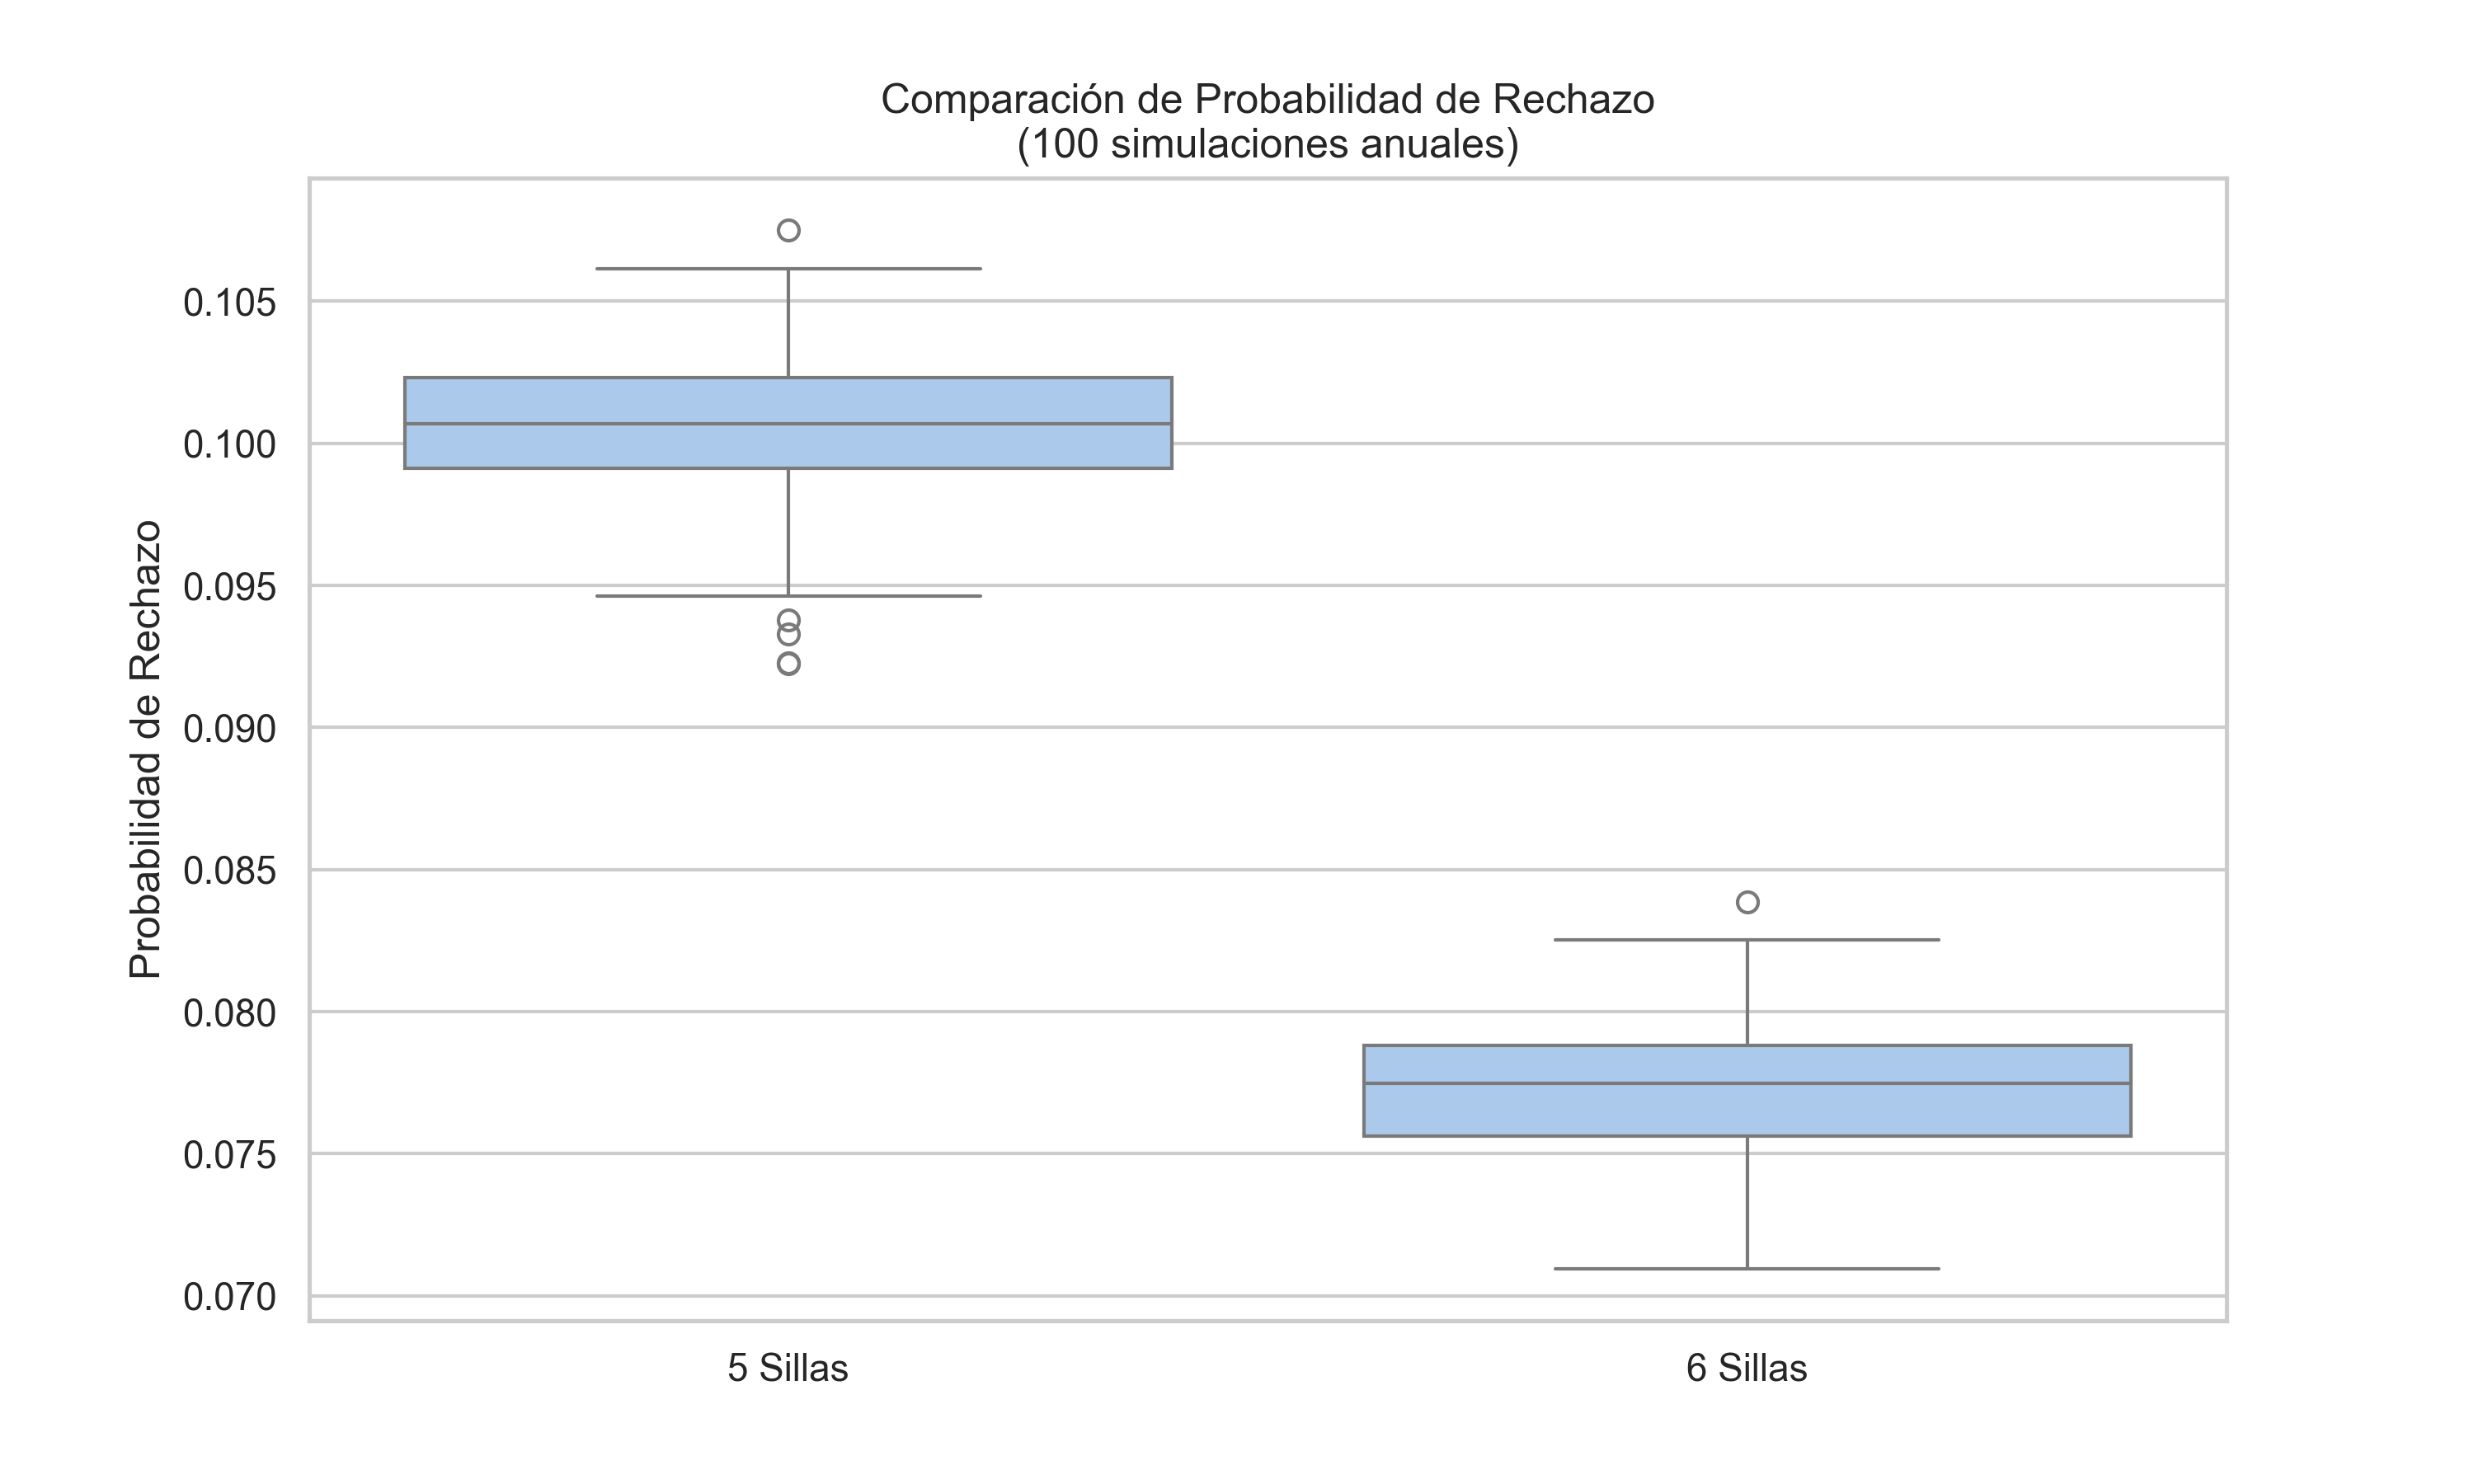
\includegraphics[width=0.75\textwidth]{../images/hipotesis_rechazo.png}
    \caption{Distribución de probabilidades de rechazo en ambas configuraciones. Se observa clara separación entre las distribuciones (solapamiento $<$ 0.1\%)}
    \label{fig:hipotesis}
\end{figure}

\subsubsection{Conclusión} 
Rechazamos $H_0$ ($p < 0.05$). La diferencia es estadística y prácticamente significativa. La reducción promedio del 6.8\% implica que por cada 100 clientes:
\begin{itemize}
    \item Se perderían $\approx$10 clientes con 5 sillas
    \item Se perderían $\approx$3 clientes con 6 sillas
\end{itemize}

\subsection{Análisis de Sensibilidad}

El análisis de sensibilidad evalúa cómo varía la probabilidad de rechazo (\(P_{\text{rechazo}}\))
al cambiar la capacidad del sistema (número de sillas disponibles). Para este análisis, se realizaron
simulaciones con capacidades que van desde 3 hasta 8 sillas, manteniendo constantes los parámetros
\(\lambda = 5\) clientes/hora y \(\mu = 6\) servicios/hora.

\subsubsection{Resultados}

En la Figura~\ref{fig:sensibilidad}, se observa cómo la probabilidad de rechazo disminuye a 
medida que aumenta el número de sillas. Esto se debe a que una mayor capacidad permite 
atender a más clientes antes de que el sistema alcance su límite.

\begin{figure}[H]
    \centering
    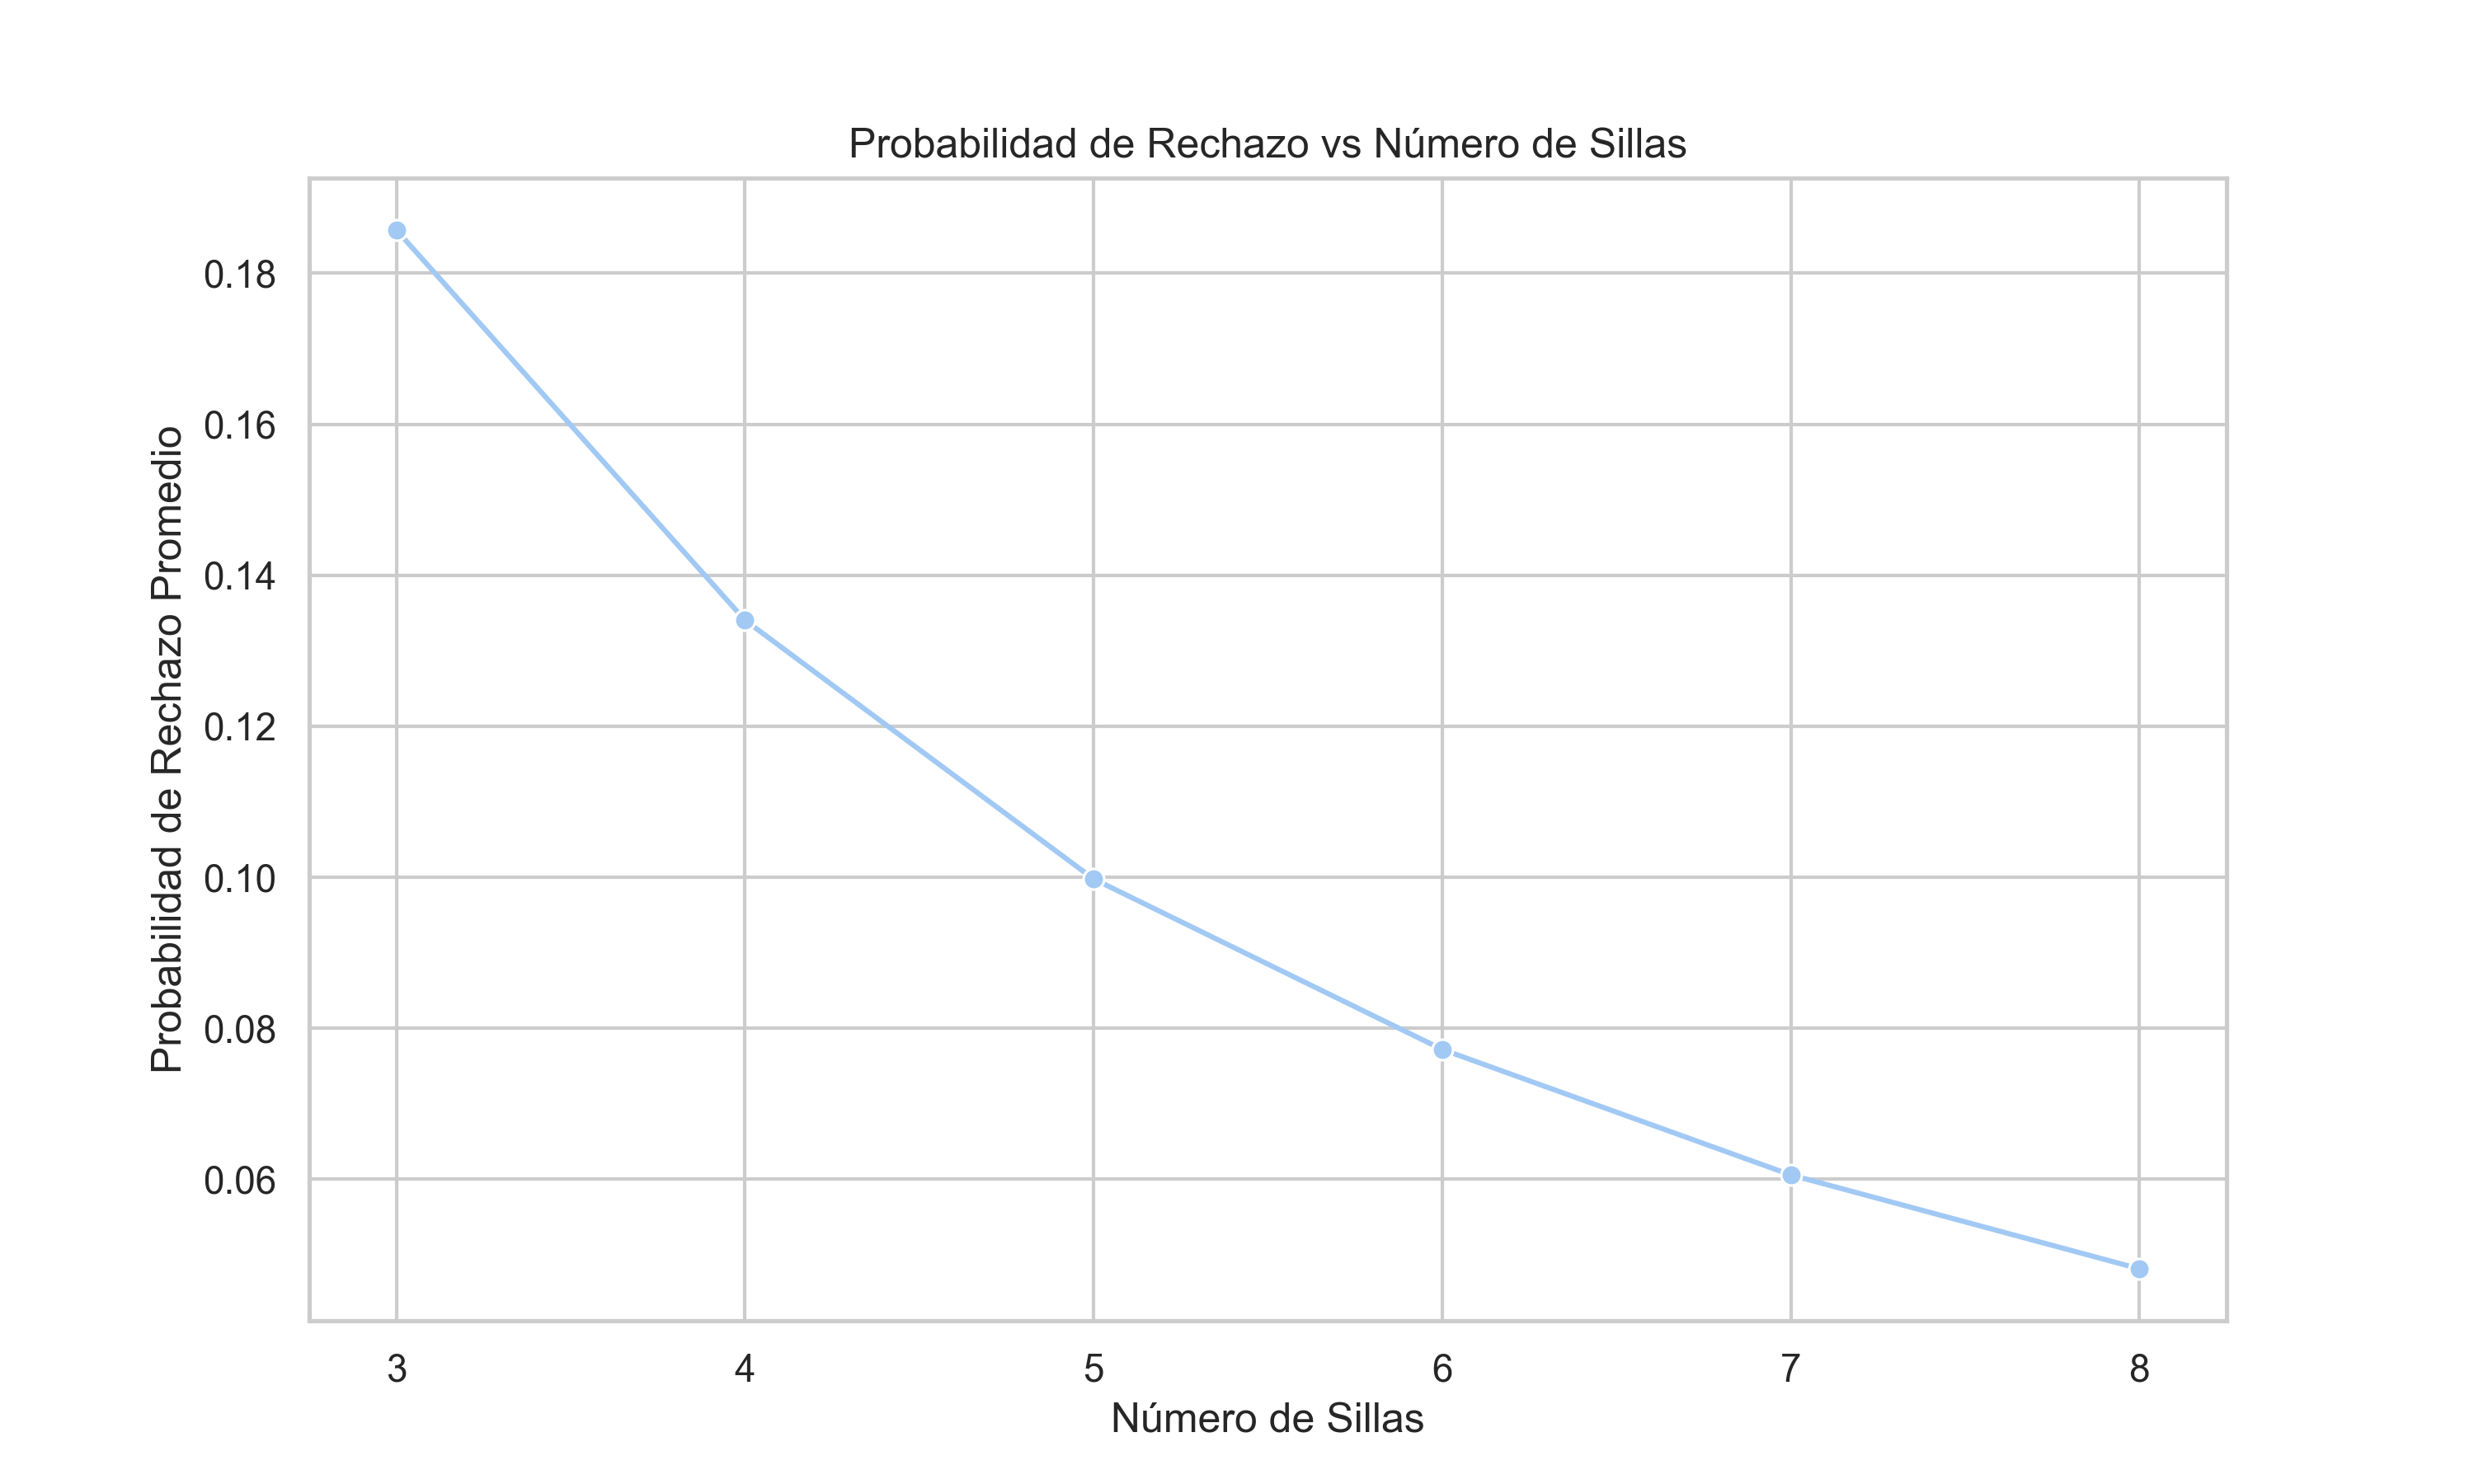
\includegraphics[width=0.8\textwidth]{../images/sensibilidad.png}
    \caption{Probabilidad de rechazo vs. número de sillas.}
    \label{fig:sensibilidad}
\end{figure}

\subsubsection{Conclusión}

El análisis muestra que aumentar la capacidad del sistema reduce significativamente la 
probabilidad de rechazo. Por ejemplo, al pasar de 5 a 6 sillas, la probabilidad de 
rechazo disminuye en un promedio del 2.33\%. 
Esto sugiere que incrementar la capacidad es una estrategia efectiva para mejorar la 
experiencia del cliente y reducir pérdidas.

\subsection{Análisis de las Distribuciones de los Tiempos de Espera}

El análisis de las distribuciones de los tiempos de espera permite evaluar cómo se comportan 
los tiempos que los clientes pasan esperando en el sistema. Este análisis es crucial para 
identificar cuántos clientes experimentan tiempos de espera prolongados y cómo estos 
tiempos afectan la experiencia del cliente.

\subsubsection{Resultados}

En la Figura~\ref{fig:distribucion_esperas}, se muestra la distribución de los tiempos de espera 
para los clientes en el sistema. Además, se incluye una línea vertical que marca el umbral de 
45 minutos, destacando el porcentaje de clientes que esperan más de este tiempo.

\begin{figure}[H]
    \centering
    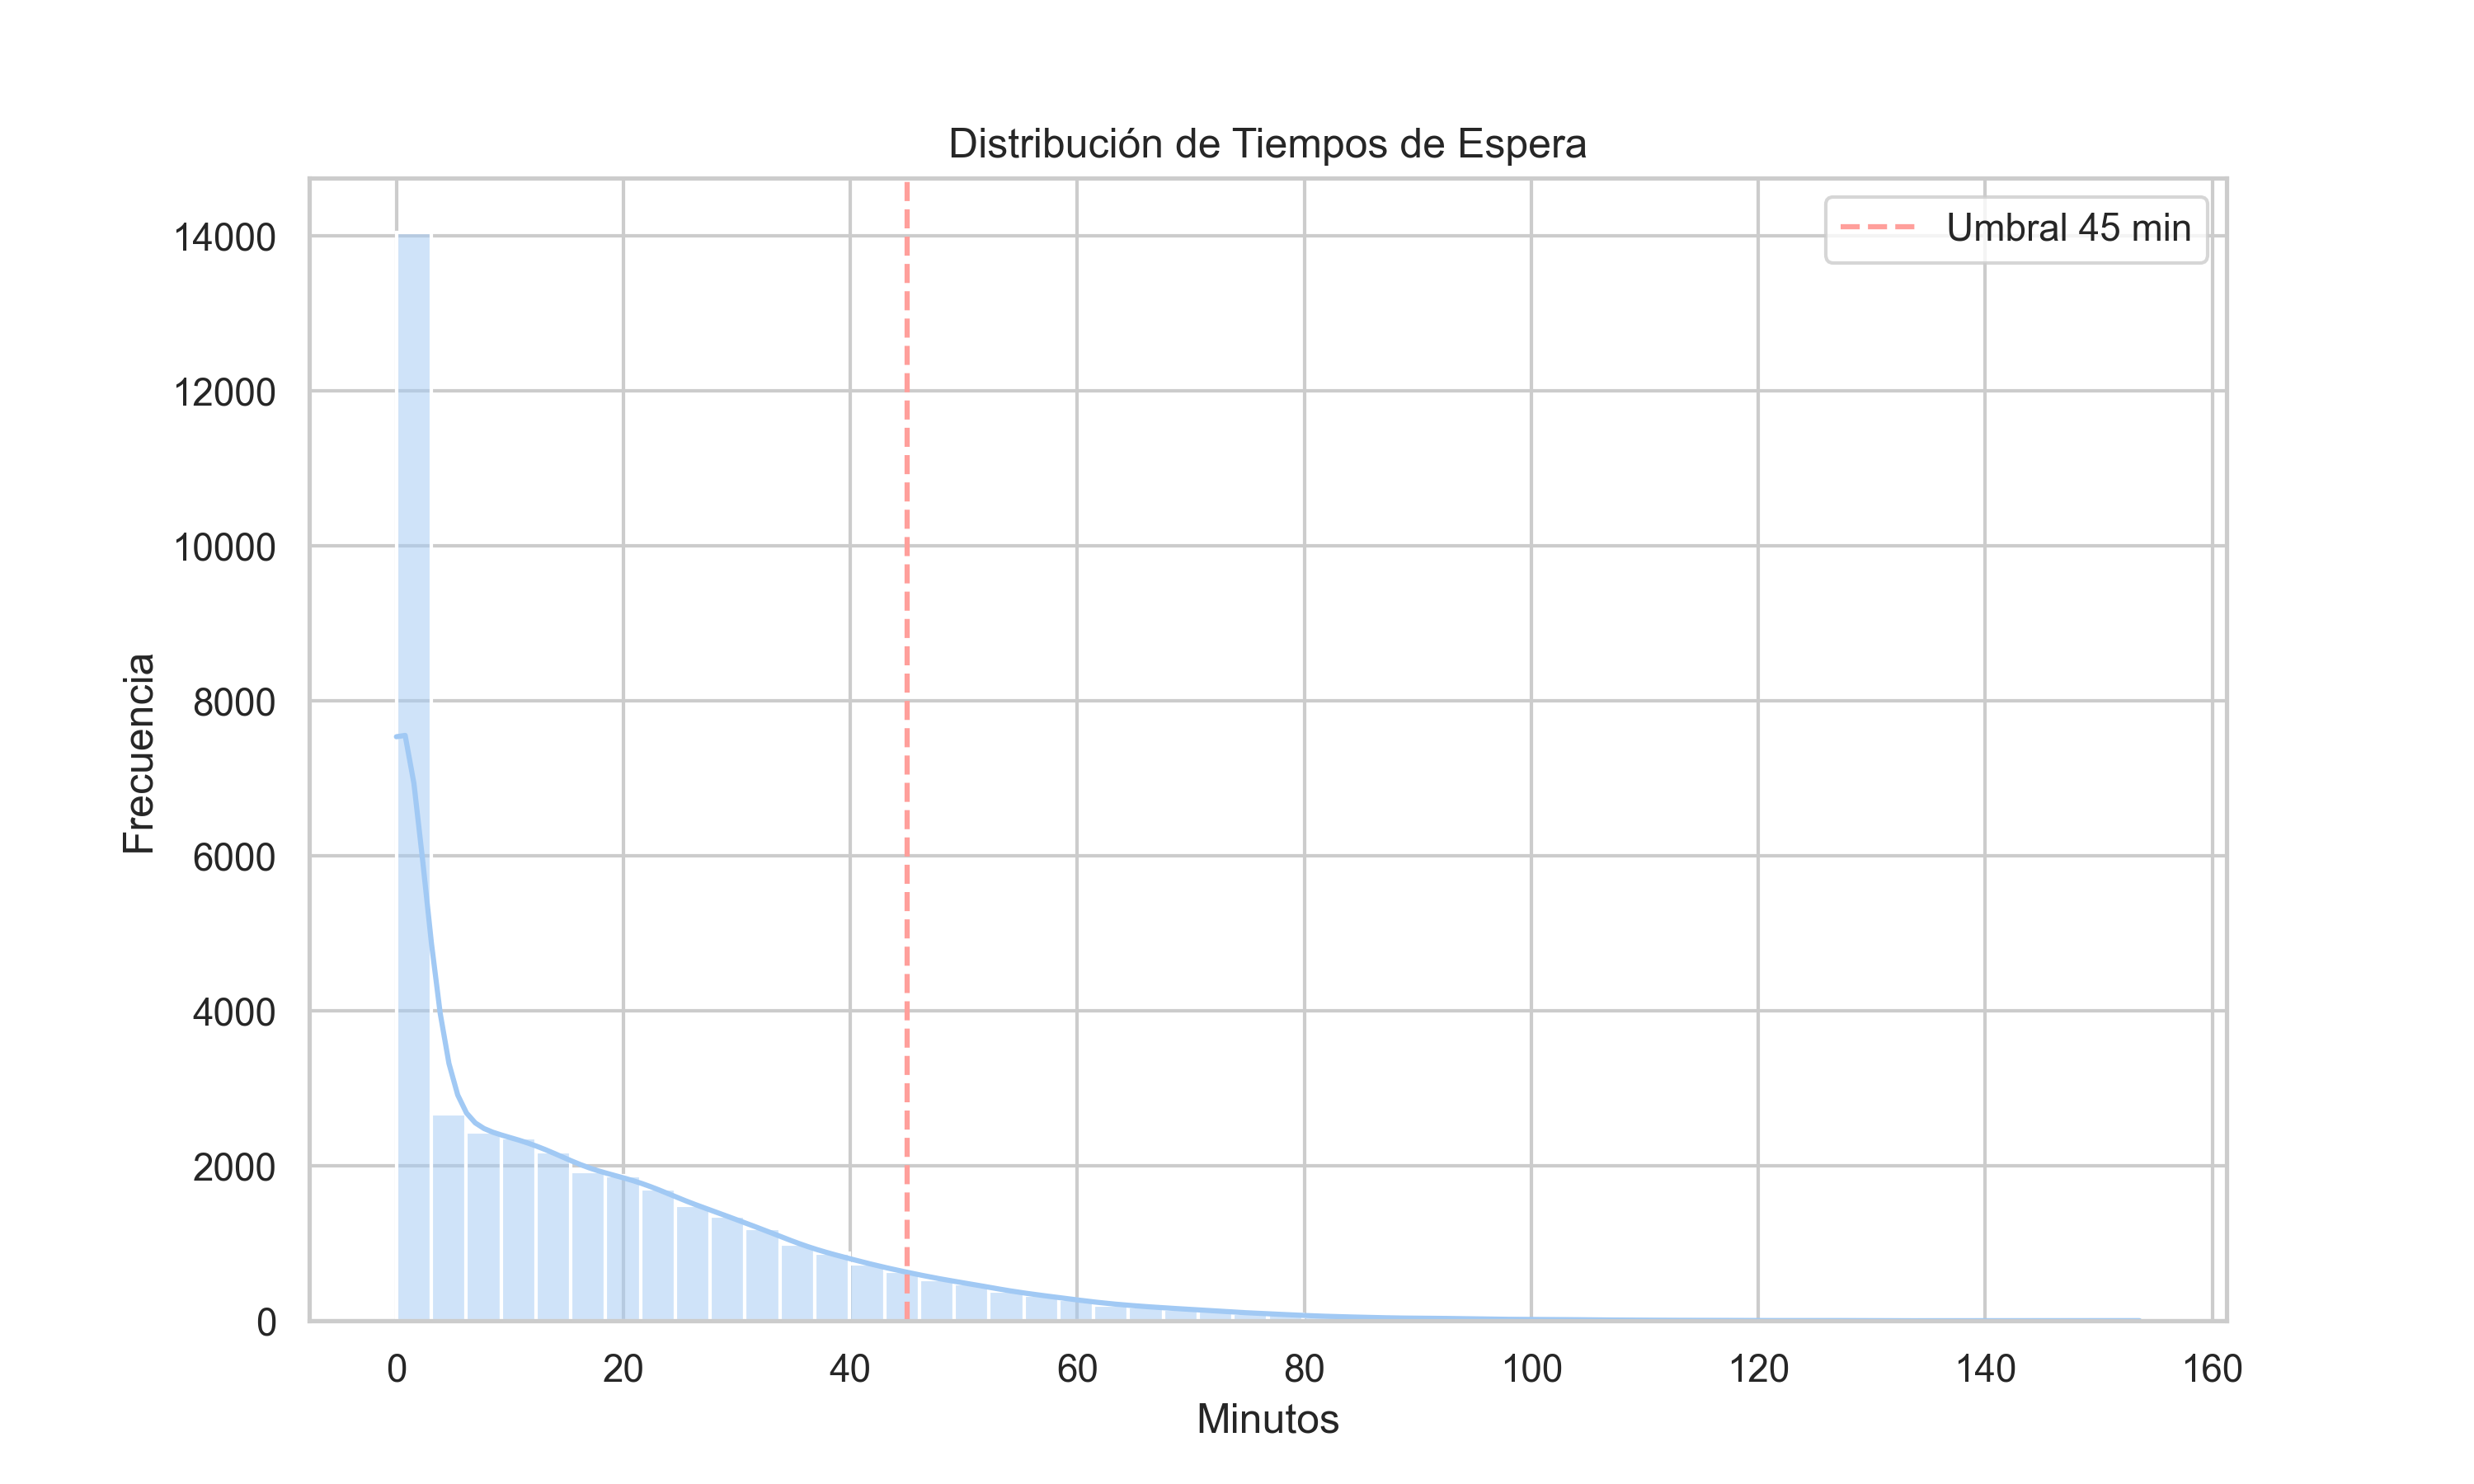
\includegraphics[width=0.8\textwidth]{../images/distribucion_esperas.png}
    \caption{Distribución de los tiempos de espera. La línea roja indica el umbral de 45 minutos.}
    \label{fig:distribucion_esperas}
\end{figure}

\subsubsection{Conclusión}

El análisis muestra que la mayoría de los clientes tienen tiempos de espera razonables, pero un 
porcentaje relativamente pequeño supera el umbral de 45 minutos. Este porcentaje puede ser reducido 
aumentando la capacidad del sistema o mejorando la tasa de servicio (\(\mu\)). Según los 
resultados de la simulación, aproximadamente el \(8.86\%\) de los clientes experimentan tiempos 
de espera superiores a 45 minutos.

\section{Modelo Matemático}
El sistema se modela como una cola \textbf{M/M/1/5} con:
\begin{itemize}
    \item Tasa de llegada $\lambda = 5$ clientes/hora (Poisson)
    \item Tasa de servicio $\mu = 6$ clientes/hora (exponencial)
    \item Capacidad $k = 5$ clientes (1 en servicio + 4 en espera)
\end{itemize}

\subsection{Parámetros Clave}
\begin{align*}
    \rho &= \frac{\lambda}{\mu} = \frac{5}{6} \approx 0.8333 \text{ (probabilidad de que el servidor esté ocupado)}\\
\end{align*}

Se define $P_n$ como la probabilidad de que hayan n clientes en el sistema.

\begin{align*}
    P_0 &= \frac{1 - \rho}{1 - \rho^k} = \frac{1 - 0.8333}{1 - 0.8333^5} \approx 0.2017
\end{align*}

\subsection{Probabilidades de Estado}
\[
P_n = P_0 \cdot \rho^n \quad \text{para } n = 0,1,\dots,5
\] Ver página 30 del libro \textit{Aplicando Teoría de Colas en Dirección de Operaciones}.

\begin{table}[H]
    \centering
    \caption{Probabilidades de estado estable}
    \begin{tabular}{cc}
        \toprule
        $n$ clientes & $P_n$ \\ 
        \midrule
        0 & 0.2017 \\ 
        1 & 0.1681 \\ 
        2 & 0.1401 \\ 
        3 & 0.1168 \\ 
        4 & 0.0973 \\ 
        5 & \textbf{0.0811} \\ 
        \bottomrule
    \end{tabular}
\end{table}

\subsection{Métricas Principales}
\begin{align*}
    L_q &= \frac{P_0 \rho}{(1 - \rho)^2} \left(1 - \rho^k - (1 - \rho)k\rho^{k-1}\right) \approx 0.6019 \text{ clientes} \\
    L &= L_q + 1 - P_k \approx 1.5208 \text{ clientes} \\
    P_{\text{rechazo}} &= P_k = P_5 \approx 8.11\% \\
    W_q &= \frac{L}{\lambda (1 - P_k)} - \frac{1}{\mu} \approx 0.1642 \text{ horas (9.85 minutos)}\\
\end{align*}

Ver página 31 del libro \textit{Aplicando Teoría de Colas en Dirección de Operaciones}.

\section{Comparación con Simulación}
\begin{table}[H]
    \centering
    \caption{Resultados analíticos vs. simulación (1 año)}
    \begin{tabular}{lSS}
        \toprule
        Métrica & {Analítico} & {Simulación} \\
        \midrule
        $L$ & 1.52 & 1.97 \\
        $L_q$ & 0.60 & 1.22 \\
        $W_q$ & 9.85 & 16.3 \\
        $P_{\text{rechazo}}$ (\%) & 8.11 & 10.00 \\
        \bottomrule
    \end{tabular}
\end{table}

Los resultados provistos por la simulación no están tan alejados de los resultados analíticos. Una forma de 
mejorar su precisión sería incrementando el tiempo de la simulación, que actualmente solo simula 8760 horas, 
equivalente a un año.

\section{Conclusiones}
\begin{itemize}
    \item La probabilidad de rechazo ($\approx$\SI{10}{\%}) sugiere que en horas pico se pierde 1 cliente cada 10.
    \item El rechazo a los clientes podría reducirse si se aumenta la cantidad de sillas en el salón.
    \item Aunque se plantea la posibilidad de contratar a una ayudante, según los resultados, no es imprescindible para el
    negocio, pues el porcentaje de clientes rechazados y el tiempo de espera de cada uno es relativamente bajo y solo agregando sillas 
    (que significa una menor inversión que contratar una ayudante) se pueden mejorar.
\end{itemize}

\end{document}